%Version 3 December 2023
% See section 11 of the User Manual for version history
%
%%%%%%%%%%%%%%%%%%%%%%%%%%%%%%%%%%%%%%%%%%%%%%%%%%%%%%%%%%%%%%%%%%%%%%
%%                                                                 %%
%% Please do not use \input{...} to include other tex files.       %%
%% Submit your LaTeX manuscript as one .tex document.              %%
%%                                                                 %%
%% All additional figures and files should be attached             %%
%% separately and not embedded in the \TeX\ document itself.       %%
%%                                                                 %%
%%%%%%%%%%%%%%%%%%%%%%%%%%%%%%%%%%%%%%%%%%%%%%%%%%%%%%%%%%%%%%%%%%%%%

%%\documentclass[referee,sn-basic]{sn-jnl}% referee option is meant for double line spacing

%%=======================================================%%
%% to print line numbers in the margin use lineno option %%
%%=======================================================%%

%%\documentclass[lineno,sn-basic]{sn-jnl}% Basic Springer Nature Reference Style/Chemistry Reference Style

%%======================================================%%
%% to compile with pdflatex/xelatex use pdflatex option %%
%%======================================================%%

%%\documentclass[pdflatex,sn-basic]{sn-jnl}% Basic Springer Nature Reference Style/Chemistry Reference Style


%%Note: the following reference styles support Namedate and Numbered referencing. By default the style follows the most common style. To switch between the options you can add or remove “Numbered” in the optional parenthesis.
%%The option is available for: sn-basic.bst, sn-vancouver.bst, sn-chicago.bst%

%%\documentclass[pdflatex,sn-nature]{sn-jnl}% Style for submissions to Nature Portfolio journals
%%\documentclass[pdflatex,sn-basic]{sn-jnl}% Basic Springer Nature Reference Style/Chemistry Reference Style
\documentclass[pdflatex,sn-nature]{sn-jnl}% Style for submissions to Nature Portfolio journals
%%\documentclass[pdflatex,sn-mathphys-num]{sn-jnl}% Math and Physical Sciences Numbered Reference Style
%%\documentclass[pdflatex,sn-mathphys-ay]{sn-jnl}% Math and Physical Sciences Author Year Reference Style
%%\documentclass[pdflatex,sn-aps]{sn-jnl}% American Physical Society (APS) Reference Style
%%\documentclass[pdflatex,sn-vancouver,Numbered]{sn-jnl}% Vancouver Reference Style
%%\documentclass[pdflatex,sn-apa]{sn-jnl}% APA Reference Style
%%\documentclass[pdflatex,sn-chicago]{sn-jnl}% Chicago-based Humanities Reference Style

%%%% Standard Packages
%%<additional latex packages if required can be included here>

\usepackage{graphicx}%
\usepackage{multirow}%
\usepackage{amsmath,amssymb,amsfonts}%
\usepackage{amsthm}%
\usepackage{mathrsfs}%
\usepackage[title]{appendix}%
\usepackage{xcolor}%
\usepackage{textcomp}%
\usepackage{manyfoot}%
\usepackage{booktabs}%
\usepackage{algorithm}%
\usepackage{algpseudocode}%
\usepackage{listings}%
\graphicspath{{figures/}}
\usepackage[superscript,biblabel]{cite}
\usepackage{float}
\usepackage{caption}
%%%%

%%%%%=============================================================================%%%%
%%%%  Remarks: This template is provided to aid authors with the preparation
%%%%  of original research articles intended for submission to journals published
%%%%  by Springer Nature. The guidance has been prepared in partnership with
%%%%  production teams to conform to Springer Nature technical requirements.
%%%%  Editorial and presentation requirements differ among journal portfolios and
%%%%  research disciplines. You may find sections in this template are irrelevant
%%%%  to your work and are empowered to omit any such section if allowed by the
%%%%  journal you intend to submit to. The submission guidelines and policies
%%%%  of the journal take precedence. A detailed User Manual is available in the
%%%%  template package for technical guidance.
%%%%%=============================================================================%%%%

%% as per the requirement new theorem styles can be included as shown below
\theoremstyle{thmstyleone}%
\newtheorem{theorem}{Theorem}%  meant for continuous numbers
%%\newtheorem{theorem}{Theorem}[section]% meant for sectionwise numbers
%% optional argument [theorem] produces theorem numbering sequence instead of independent numbers for Proposition
\newtheorem{proposition}[theorem]{Proposition}%
%%\newtheorem{proposition}{Proposition}% to get separate numbers for theorem and proposition etc.

\theoremstyle{thmstyletwo}%
\newtheorem{example}{Example}%
\newtheorem{remark}{Remark}%

\theoremstyle{thmstylethree}%
\newtheorem{definition}{Definition}%

\raggedbottom
\unnumbered% uncomment this for unnumbered level heads

\begin{document}

\title[Article]{Large Language Model Consensus Substantially Improves the Cell Type Annotation Accuracy for scRNA-seq Data}

\author[1]{\fnm{Chen} \sur{Yang}}\email{cafferychen777@tamu.edu}

\author*[1]{\fnm{Xianyang} \sur{Zhang}}\email{zhangxiany@stat.tamu.edu}

\author*[2]{\fnm{Jun} \sur{Chen}}\email{Chen.Jun2@mayo.edu}

\affil*[1]{\orgdiv{Department of Statistics}, \orgname{Texas A\&M University}, \orgaddress{\city{College Station}, \state{Texas}, \postcode{77843}, \country{USA}}}

\affil[2]{\orgdiv{Division of Computational Biology, Department of Quantitative Health Sciences}, \orgname{Mayo Clinic}, \orgaddress{\city{Rochester}, \state{Minnesota}, \postcode{55905}, \country{USA}}}

%%==================================%%
%% Sample for unstructured abstract %%
%%==================================%%

\abstract{The rapid expansion of single-cell RNA sequencing (scRNA-seq) has made accurate cell type annotation a critical bottleneck for biological discovery. Existing computational methods are often limited by reference data dependency, while emerging single Large Language Model (LLM) approaches are susceptible to model-specific biases and provide insufficient uncertainty quantification. To address these limitations, we introduce mLLMCelltype, a framework that harnesses collective intelligence—the emergent problem-solving capacity arising when multiple independent agents interact through structured deliberation to produce solutions exceeding individual capabilities—of multiple LLMs through an iterative deliberation process. Across 49 diverse datasets, our framework achieves a mean accuracy of 77.2\%, a 15.7-percentage-point improvement over the best-performing single-LLM baseline (61.5\%). The consensus mechanism demonstrates high robustness to noisy input and generalizes to datasets released after the LLMs' training. By providing transparent reasoning chains and robust consensus-based confidence metrics, mLLMCelltype minimizes manual annotation effort and enables reliable interpretation of complex cellular landscapes. The framework is available as an open-source package and an accessible web server.}

\keywords{Cell type annotation, Collective intelligence, Large language models, Multi-LLM consensus, scRNA-seq, Uncertainty quantification}

%%\pacs[JEL Classification]{D8, H51}

%%\pacs[MSC Classification]{35A01, 65L10, 65L12, 65L20, 65L70}

\maketitle

\section{Introduction}

The widespread adoption of single-cell RNA sequencing (scRNA-seq) has generated cellular data at a rapidly expanding scale, with large-scale consortia such as the Human Cell Atlas producing reference maps containing millions of cells\cite{sikkemaIntegratedCellAtlas2023}. A primary bottleneck in translating this data into biological knowledge is cell type annotation, the process of assigning cellular identities based on gene expression profiles\cite{pasquiniAutomatedMethodsCell2021}. While manual annotation by human experts remains a gold standard, it is slow, requires deep domain expertise, and does not scale effectively to the rapidly growing number and diversity of datasets—even annotating dozens of clusters across multiple studies and tissue types requires substantial expert time and specialized knowledge, creating a demand for accurate and automated computational methods.

Over the past decade, numerous computational tools have been developed for this purpose\cite{chengReviewSinglecellRNAseq2023}. These methods broadly fall into three categories. Supervised, reference-mapping methods such as SingleR\cite{aran2019reference} and Seurat\cite{stuart2019comprehensive} achieve high accuracy when a well-matched, comprehensive reference atlas is available. However, recent benchmarking studies show that while performance can be high on simpler datasets, it often drops significantly on complex atlases with many fine-grained cell types. For example, a 2024 benchmark analysis demonstrated that while several methods performed well on broad cell type classification, their F1-scores for distinguishing 20 closely related T-cell subtypes were often around 0.83-0.84\cite{Yuan2024scRGCL}, highlighting the persistent challenge of high-resolution annotation. Furthermore, these methods operate under a "closed-world" assumption and are prone to misclassifying cell types or states that are absent from the reference\cite{cao2022openworld}, a critical limitation for studying previously uncharacterized biological systems or disease states. Semi-supervised approaches like SCINA\cite{zhang2019scina} leverage prior knowledge of cell type-specific gene signatures combined with expectation-maximization algorithms, offering a middle ground between the rigid constraints of reference mapping and the flexibility of unsupervised methods. Conversely, unsupervised methods like scCATCH\cite{shao2020sccatch} rely on matching marker gene lists against databases. While this approach avoids direct dependency on a reference transcriptome atlas, it utilizes only a fraction of the available transcriptomic information and often fails to distinguish between cell subtypes with subtle expression differences or overlapping markers\cite{luecken2021benchmarking}.

The emergence of transformer-based foundation models, such as scBERT\cite{yang2022scbert} and scGPT\cite{cui2024scgpt}, marked a significant advance by pre-training on millions of cells to learn fundamental gene regulatory patterns. Building on this, general-purpose Large Language Models (LLMs) offer a distinct, knowledge-driven approach. Unlike foundation models that learn from expression data alone, LLMs like those in the GPT series can interpret marker gene lists by drawing on the extensive biological knowledge from the scientific literature encoded during their training\cite{houAssessingGPT4Cell2024}. Recent work has demonstrated the potential of LLMs for automated annotation: scExtract leverages LLMs to extract information from research articles for fully automated data processing and annotation\cite{wu2025scextract}, while CASSIA employs a multi-agent LLM system with explicit validation and quality scoring mechanisms to address hallucination concerns\cite{xie2024cassia}. However, relying on any single model—whether a specialized foundation model or a general-purpose LLM—introduces critical vulnerabilities. First, every model has inherent biases resulting from its specific training data and architecture, which can lead to systematic errors. Second, single LLMs are prone to ``hallucination''—generating plausible but factually incorrect biological reasoning, a challenge that persists even in systems with validation layers\cite{xie2024cassia}. Finally, a single model cannot provide robust uncertainty metrics based on peer disagreement, making it difficult to identify and flag annotations that require expert review.

Inspired by advances in agentic AI and multi-agent systems (MAS), where multiple AI agents collaborate to solve problems beyond the capability of any single agent\cite{duImprovingFactualityReasoning2023}, we hypothesized that a framework built on the consensus of a diverse ensemble of LLMs could mitigate these individual weaknesses. Recent developments in multi-agent frameworks for single-cell analysis, such as CellAgent's hierarchical agent architecture for automated pipeline execution\cite{xiao2024cellagent} and CASSIA's functionally specialized agents for annotation validation\cite{xie2024cassia}, have demonstrated the value of agent collaboration in biological data analysis. However, these approaches employ agents with fixed, predefined roles rather than peer deliberation, and simple ensemble or voting strategies aggregate independent predictions without allowing models to refine their reasoning in light of alternative perspectives. In contrast, our approach treats each LLM as an equal peer in an iterative deliberation process, where dynamic response diversity emerges naturally from structured argumentation rather than from static model diversity or predetermined agent functions. To test this, we developed mLLMCelltype, a framework that uses iterative, structured deliberation among multiple LLMs. The design is motivated by the Diversity Prediction Theorem\cite{Page2007TheDifference}, which shows that ensemble accuracy improves with predictor diversity---a principle our saturation analysis empirically confirms for LLM-based annotation. By enabling models to cross-validate reasoning, challenge initial hypotheses, and converge on a consensus, the framework leverages this diversity to produce annotations more accurate than those of any individual model. In this article, we demonstrate that mLLMCelltype substantially improves annotation accuracy over single-LLM methods, provides transparent uncertainty quantification to guide expert review, and maintains robustness across a wide range of tissues and data qualities.

\section{Results}

\subsection{The mLLMCelltype framework enables consensus through deliberation}
The mLLMCelltype framework integrates multiple LLMs to annotate cell types from scRNA-seq data through a structured, multi-stage process (Fig.~1). The process begins with identifying marker genes for each cell cluster from pre-processed scRNA-seq data (Fig.~1b). These marker lists, along with tissue context, are provided as input to an ensemble of diverse LLMs (Fig.~1c-d). Each LLM independently proposes an initial annotation. For clusters where models disagree, the framework initiates an iterative deliberation process. During these rounds, LLMs share their reasoning, re-evaluate evidence based on arguments from their peers, and refine their predictions (Fig.~1e). A dedicated Consensus Checker LLM assesses the level of agreement after each round. This process continues until a predefined consensus threshold is met or a maximum number of rounds is reached, yielding a final annotation, a detailed reasoning history, and quantitative uncertainty metrics (Fig.~1f).

\begin{figure}[!htbp]
    \centering
    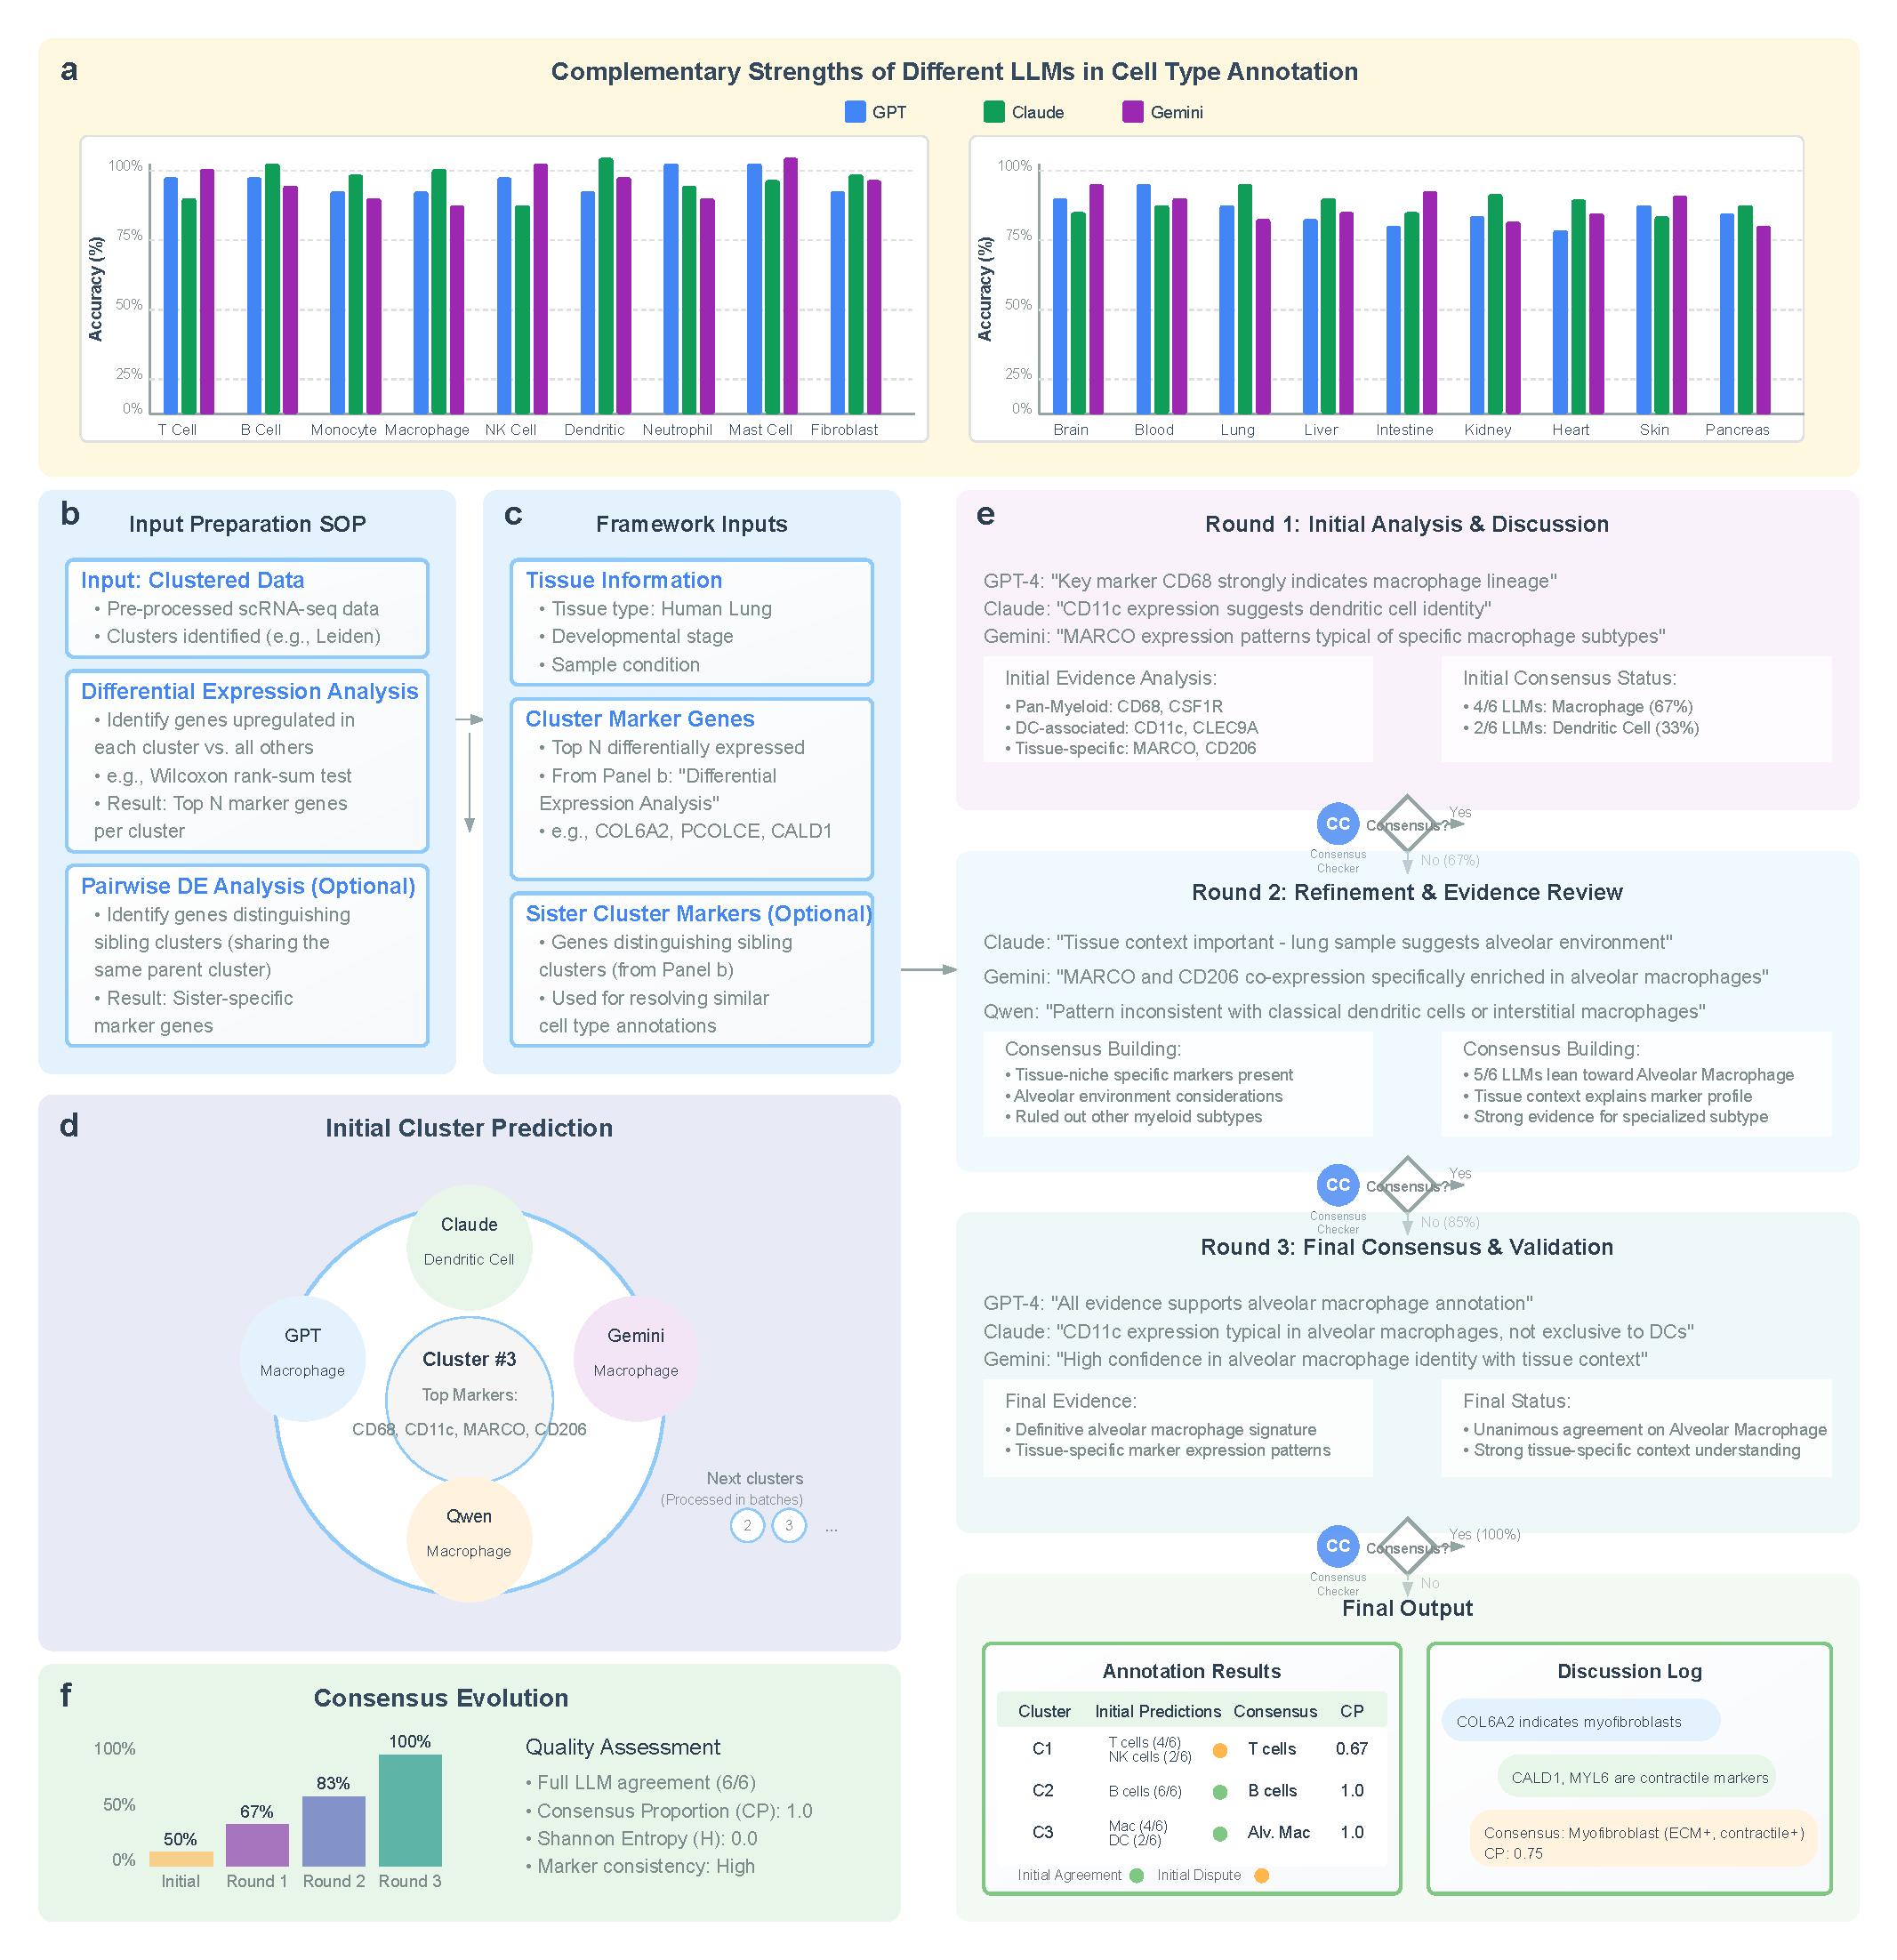
\includegraphics[width=\textwidth]{figures/figure1.pdf}
    \caption{The mLLMCelltype framework workflow.
    \textbf{a}, Complementary strengths: Different LLMs (GPT, Claude, Gemini) show varying performance across cell types and tissues, highlighting the value of a multi-model approach. The results are based on the benchmark datasets in Fig.~2a.
    \textbf{b}, Input preparation: Differential expression (DE) analysis on clustered data yields marker genes (optional: sister cluster markers).
    \textbf{c}, Framework input: Marker genes (from \textbf{b}) and tissue context are provided to the LLMs.
    \textbf{d}, Initial cluster prediction:  LLMs independently propose initial annotations per cluster based on the input.
    \textbf{e}, Iterative consensus: LLMs deliberate over multiple rounds, sharing arguments under the guidance of a Consensus Checker (CC) to reach an agreement. Output includes the final annotation and Consensus Proportion (CP).
    \textbf{f}, Consensus evolution: Deliberation progressively improves consensus over successive rounds.
}\label{fig:workflow}
\end{figure}

\subsection{Consensus among multiple LLMs improves annotation accuracy}
Our central hypothesis is that aggregating knowledge from a diverse set of LLMs can lead to higher accuracy than relying on any single model. To test this, we systematically evaluated the impact of the number of participating LLMs on performance using the Tabula Sapiens dataset. As shown in Fig.~2a, annotation accuracy steadily increases with the addition of more LLMs to the consensus process, rising from an average of 59.3\% with a single LLM to 75.8\% with an ensemble of six. This demonstrates that different models provide complementary knowledge, and their collective assessment is more accurate. Critically, this improvement is most pronounced for cell clusters that are difficult to annotate. For clusters where the best single LLM performed poorly ($<$60\% initial accuracy), the six-LLM consensus framework improved accuracy by 38\% (Fig.~2b). This highlights the value of the ensemble approach for resolving challenging annotation cases.

\begin{figure}[!htbp]
    \centering
    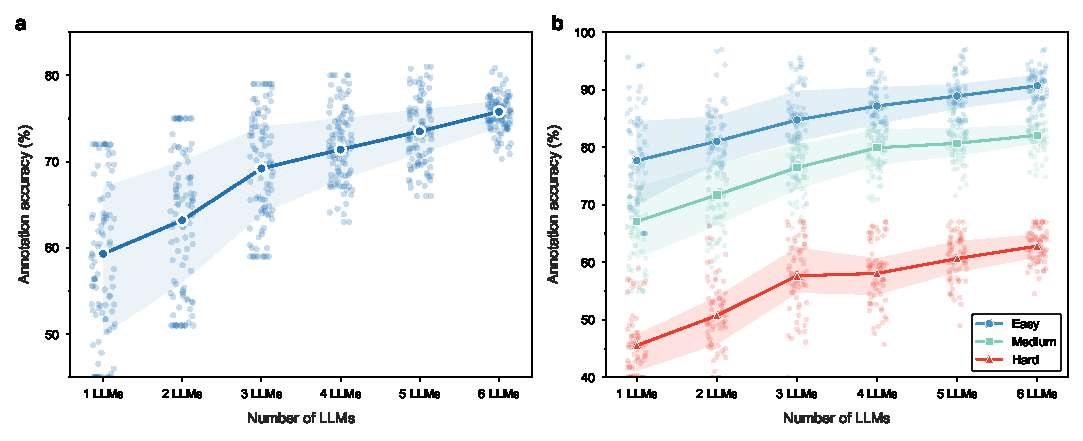
\includegraphics[width=\textwidth]{figures/figure2.pdf}
    \caption{Consensus among multiple LLMs improves annotation accuracy.
    \textbf{a}, Relationship between the number of participating LLMs (1 to 6) and the overall mean annotation accuracy across all clusters using the Tabula Sapiens (TS) dataset. The line plot shows a consistent improvement in accuracy as more LLMs are added to the consensus process. For "1 LLM", we computed the average performance across all six individual LLMs when used alone (without deliberation), with each LLM evaluated independently. For "2 LLMs", "3 LLMs", etc., we randomly sampled LLM combinations (without replacement) from the full set of six models. The shaded area represents the standard deviation based on 100 independent runs for each number of LLMs (for "1 LLM": 100 runs per individual model, then averaged across all 6 models; for "2-6 LLMs": 100 random combinations sampled and evaluated), illustrating reduced variability and increased result stability with larger ensembles.
    \textbf{b}, Annotation accuracy improvement varies with cluster annotation difficulty. Clusters from the TS dataset were categorized into 'Easy', 'Medium', and 'Hard' based on the initial annotation accuracy achieved by the single best-performing LLM (Easy: $>$85\% initial accuracy; Medium: 60-85\%; Hard: $<$60\%). The plots show accuracy trends for each difficulty category as the number of LLMs increases. While 'Easy' clusters reach high accuracy quickly, 'Medium' and 'Hard' clusters show the most significant relative gains from ensemble consensus (+22.4\% and +38.0\% accuracy improvement respectively, going from 1 to 6 LLMs), highlighting the value of multi-LLM deliberation for challenging annotations.
    }
    \label{fig:llm_number_impact}
\end{figure}

\subsection{Iterative deliberation actively reduces model errors and enhances reliability}
The mLLMCelltype framework improves accuracy not just by simple ensembling, but through an active error-correction mechanism analogous to multi-agent debate\cite{duImprovingFactualityReasoning2023}. To investigate this, we quantified the rate of "hallucinations"—annotations that are biologically implausible or contradicted by the provided marker gene evidence. In the initial round of predictions, a notable fraction of annotations were classified as hallucinations. However, this fraction decreased substantially with each subsequent round of deliberation, as models corrected their initial assessments based on the arguments of others (Fig.~3a). This observation aligns with findings in MAS research, where mutual criticism among agents has been shown to reduce factual errors and hallucinations\cite{duImprovingFactualityReasoning2023}. Furthermore, the strong correlation between consensus proportion and annotation reliability (Fig.~3b) suggests that inter-agent agreement serves as a robust proxy for confidence, a key feature of reliable collective intelligence systems. The pairwise concordance between models also progressively increases across deliberation rounds, signifying convergence towards a well-reasoned consensus (Supplementary Fig.~1).

\begin{figure}[!htbp]
    \centering
    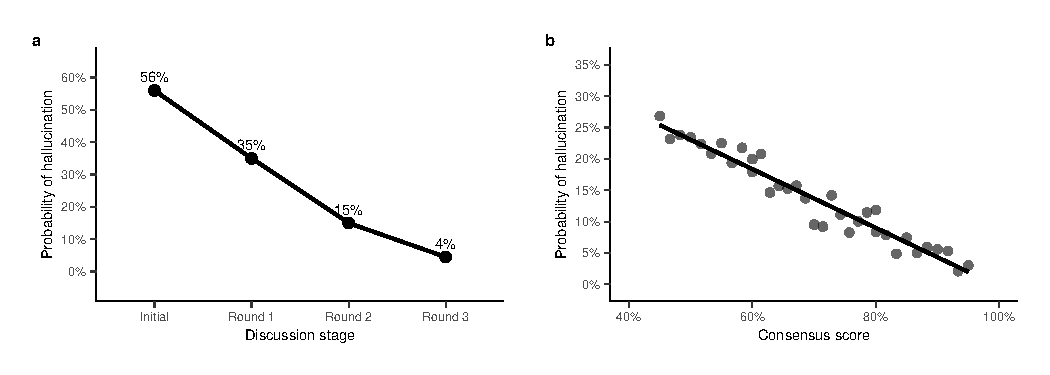
\includegraphics[width=\textwidth]{figures/figure3.pdf}
    \caption{Iterative deliberation actively reduces model errors and enhances reliability.
    \textbf{a}, Progressive reduction in the proportion of annotations classified as hallucinations across deliberation rounds based on analysis of the Tabula Sapiens (TS) dataset. In the context of cell type annotation, hallucination refers to LLM-generated annotations or interpretations that are: 1) contradicted by the provided marker gene evidence (e.g., assigning a T cell identity despite lacking key T cell markers like CD3D), 2) inconsistent with established cell type ontologies (e.g., claiming a cell is simultaneously a B cell and a T cell), or 3) biologically implausible given the tissue context (e.g., identifying neurons in a pure immune cell dataset). Annotations were manually reviewed against these criteria to determine hallucination status. The proportion of annotations identified as hallucinations decreases substantially from the initial predictions (Round 0) through subsequent rounds of structured deliberation, demonstrating the error-correcting effect of the consensus process.
    \textbf{b}, Negative correlation between consensus proportion and the likelihood of hallucination. Each point represents a single cell cluster from the TS dataset. Clusters are grouped by their final consensus proportion (x-axis), and the y-axis shows the proportion of clusters within that group whose final consensus annotation was classified as a hallucination based on the criteria in (a). Higher consensus proportion among models strongly correlates with a lower likelihood of the final annotation being a hallucination, indicating increased reliability. Conversely, low consensus flags clusters where annotations are less certain and may require expert review.
    }
    \label{fig:hallucination_reduction}
\end{figure}

\subsection{mLLMCelltype demonstrates superior performance across diverse benchmarks}
We benchmarked mLLMCelltype against established cell type annotation methods representing different computational paradigms: scType\cite{ianevski2022fully} (a marker-based method), SingleR\cite{aran2019reference} (a reference-based method), GPTCelltype (a single-LLM method), popV (a machine learning-based consensus method), and scANVI\cite{xu2021probabilistic} (a classification-based method). Across 49 datasets, mLLMCelltype achieved a mean annotation accuracy of 77.2\%, substantially outperforming all baseline methods. The improvement over GPTCelltype (61.5\%, +15.7 percentage points) confirms that the deliberation process among multiple LLMs, rather than single-model querying, is essential for maximizing accuracy. We additionally compared against scANVI, a classification-based method that requires per-dataset training on a labeled reference atlas. Across the 7 popV benchmark datasets, mLLMCelltype outperformed scANVI on 5 of 7 datasets (mean accuracy 71.6\% vs.\ 56.7\%), with particularly large advantages on datasets where the reference lacked cell types present in the query (Supplementary Fig.~8a). On the subset of datasets where reference-based evaluation was feasible (see Methods), mLLMCelltype also substantially outperformed SingleR and scType using Cell Ontology-aware accuracy scoring, demonstrating advantages over both dominant annotation paradigms (Supplementary Fig.~9, Supplementary Data~2). Because cell types form a taxonomic hierarchy in the Cell Ontology, we additionally assessed performance with hierarchical precision, recall, and F1 metrics\cite{kosmopoulos2015evaluation} that give partial credit for predictions close to the correct type in the ontology: mLLMCelltype achieved macro-averaged hP\,=\,0.89, hR\,=\,0.88, and hF1\,=\,0.88, compared to GPTCelltype's hP\,=\,hR\,=\,hF1\,=\,0.75 (Supplementary Data~2). The performance gains were consistent across a wide range of tissues. For instance, on a developmental human thymus cell atlas, mLLMCelltype correctly distinguished fine-grained T-cell progenitor states that were confounded by other methods, leading to a 10.6\% accuracy improvement over popV (Fig.~4b). Similarly, in the Lung Cell Atlas (LCA), our framework achieved a 13.2\% higher accuracy by better resolving closely related pulmonary cell subsets (Fig.~4c). This ability to resolve fine-grained subtypes is a key advantage of the deliberation process. For example, in the HLCA dataset, our framework correctly identified a cluster as 'Alveolar Macrophages' by reasoning about the co-expression of specific markers like MARCO and FABP4, whereas single-LLM approaches often provided a less specific 'Macrophage' label based only on general markers like CD68. This demonstrates how deliberation leads to more precise and biologically meaningful annotations. These results show the practical benefits of the multi-LLM deliberation process on large and complex biological datasets. Per-dataset accuracy for all methods, including SingleR, scType, and the naive baseline, is visualized in Supplementary Fig.~9 and tabulated in Supplementary Data~2.

\begin{figure}[!htbp]
    \centering
    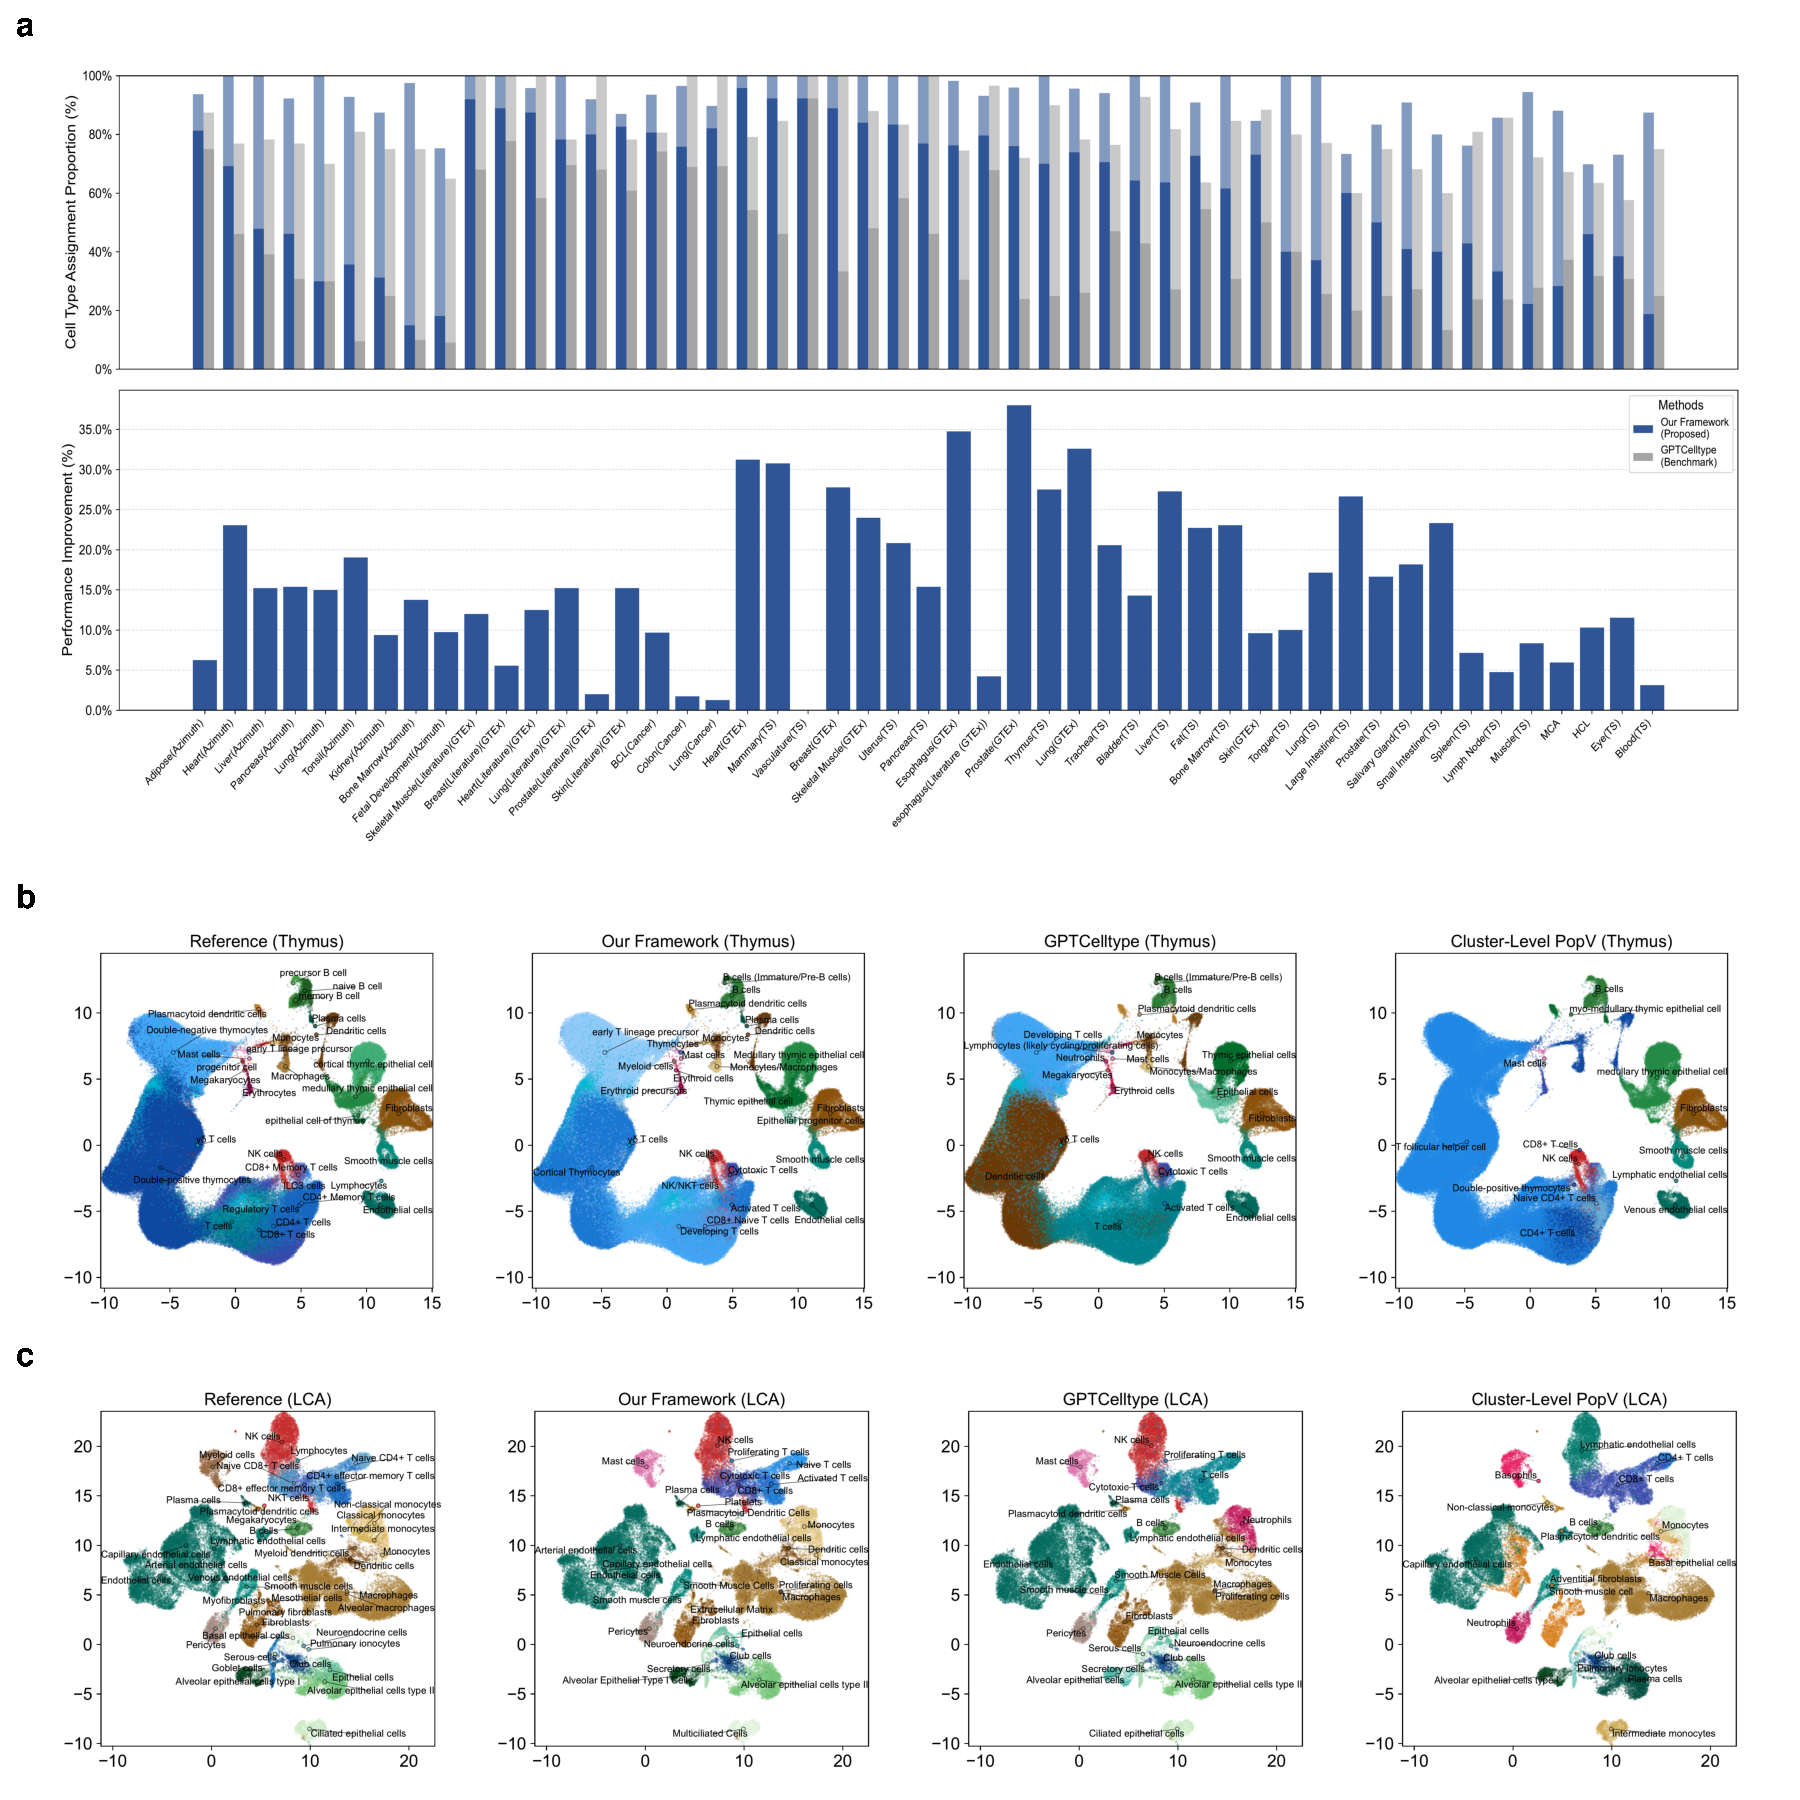
\includegraphics[width=\textwidth]{figures/figure4.pdf}
    \caption{Performance evaluation across diverse benchmarks.
    \textbf{a}, Comparison with GPTCelltype across 49 benchmark datasets. For each dataset, stacked bars show annotation accuracy as percentages. Dark-colored segments represent exact matches (predicted cell type exactly matches reference annotation), while light-colored segments represent partial matches (predicted cell type is hierarchically related to reference, e.g., predicting "T cell" when reference is "CD8+ T cell"). See Methods section for formal definitions of exact and partial match criteria.
    \textbf{b}, Performance comparison on the developmental human thymus cell atlas \cite{doi:10.1126/science.aay3224}. UMAP visualizations show cell type annotations from Reference (first), mLLMCelltype prediction (second), GPTCelltype prediction (third), and cluster-level popV prediction using Tabula Sapiens Thymus as reference (fourth), with points colored by cell type.
    \textbf{c}, Performance comparison on the Lung Cell Atlas (LCA) \cite{sikkemaIntegratedCellAtlas2023}. UMAP visualizations show cell type annotations from Reference (first), mLLMCelltype prediction (second), GPTCelltype prediction (third), and cluster-level popV prediction using Tabula Sapiens Lung as reference (fourth), colored by cell type.
    }
    \label{fig:benchmarks}
\end{figure}

\subsection{The framework is robust to noisy input and generalizes to unseen data}
A critical requirement for any annotation tool is robustness to imperfect input data. We systematically tested mLLMCelltype's performance under four types of marker gene list perturbations using the HNOCA dataset as a challenging test case (Supplementary Fig.~2): injection of housekeeping genes, injection of wrong cell-type markers, random gene injection, and random marker gene loss. Our framework demonstrated high resilience across all conditions. For example, even when 30\% of marker genes were replaced with misleading markers from a different cell type, mLLMCelltype's accuracy decreased by only 30\%, compared to a nearly 50\% drop for GPTCelltype (Fig.~5a). This robustness is critical for real-world applications where marker gene lists are often imperfect.

Analysis of performance across cell type complexity revealed that rare cell types are particularly vulnerable to noisy input, with accuracy dropping more steeply than for major cell types or common subtypes (Fig.~5b). Interestingly, the framework exhibited adaptive behavior under increasing noise, with the average number of deliberation rounds increasing from approximately 1.5 at 0\% noise to nearly 5 rounds at 50\% noise (Fig.~5c), reflecting the system's built-in quality control mechanism that triggers additional discussion when initial predictions are uncertain. However, we observed a counterintuitive pattern in the decision type distribution: at very high noise levels (40-50\%), the proportion of "Uncertain" decisions decreased rather than increased, with more clusters receiving direct consensus classifications (Fig.~5d). Investigation revealed that when marker gene quality is severely degraded, all LLMs tend to converge on broader, more conservative cell type categories (e.g., "T cell" rather than "CD8+ effector memory T cell"), producing spuriously high consensus. This highlights an important limitation: high consensus proportion does not necessarily indicate high confidence when input data quality is poor, and users should consider data quality metrics alongside consensus scores when interpreting results.

\begin{figure}[!htbp]
    \centering
    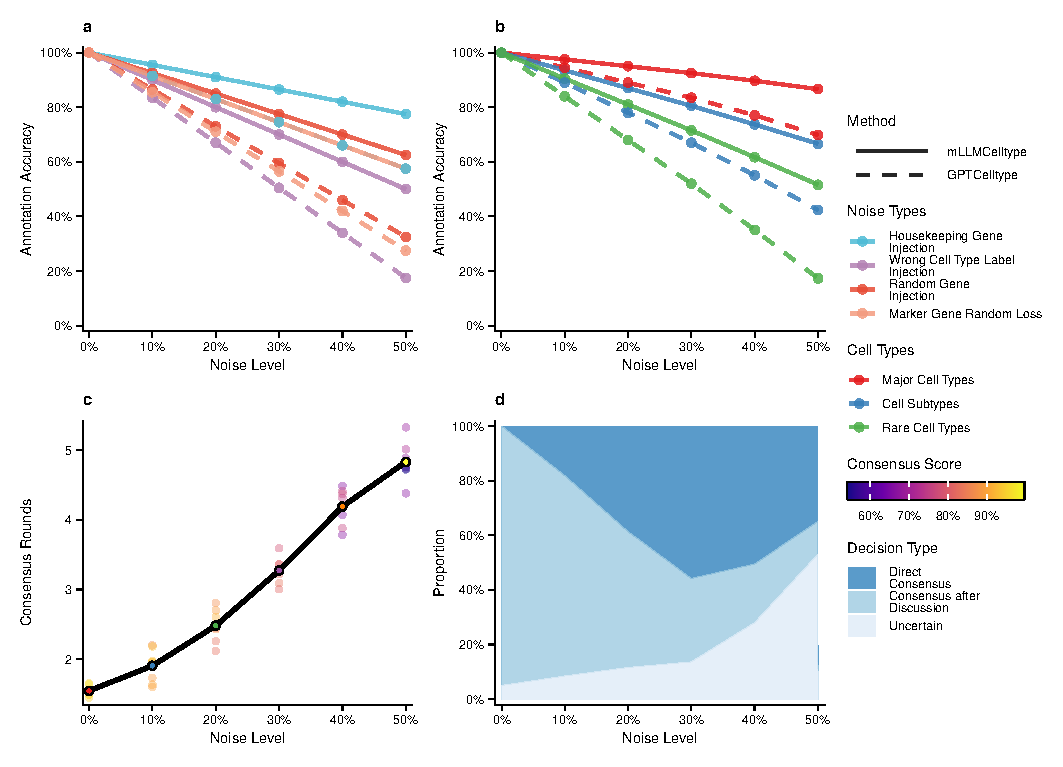
\includegraphics[width=\textwidth]{figures/figure5.pdf}
    \caption{The mLLMCelltype framework is robust to noisy marker gene input.
    \textbf{a}, Comparison of annotation accuracy robustness between mLLMCelltype (solid lines) and GPTCelltype (dashed lines) under four types of marker gene perturbations using the Human Neural Organoid Cell Atlas (HNOCA) dataset. Our framework consistently exhibited greater robustness across all perturbation types: housekeeping gene injection (blue), wrong cell type marker injection (purple), random gene injection (red), and marker gene loss (yellow). For example, under wrong cell type marker injection at 30\% noise, mLLMCelltype accuracy decreased by approximately 30\%, compared to a 49.5\% decrease for GPTCelltype.
    \textbf{b}, Performance degradation stratified by cell type complexity. Rare cell types (green) show steeper accuracy decline under noise compared to major cell types (red) and cell subtypes (blue), with both methods (solid: mLLMCelltype; dashed: GPTCelltype) showing similar trends but mLLMCelltype maintaining superior performance across all categories.
    \textbf{c}, Adaptive deliberation response to noise. The number of consensus rounds increases systematically with noise level, from approximately 1.5 rounds at 0\% noise to nearly 5 rounds at 50\% noise. Points are colored by consensus score (purple to yellow indicating 60-90\% consensus), demonstrating the framework's built-in quality control mechanism that triggers additional deliberation rounds when facing uncertain inputs.
    \textbf{d}, Decision type distribution across noise levels. Stacked areas show the proportion of clusters receiving different decision outcomes: Direct Consensus (dark blue), Consensus (medium blue), Consensus after Discussion (light blue), and Uncertain (lightest blue). Note the counterintuitive reduction in "Uncertain" decisions at very high noise levels (40-50\%), which occurs because severely degraded marker gene quality causes all LLMs to retreat to broader, more conservative cell type categories (e.g., agreeing on "T cell" rather than disagreeing on specific subtypes), producing spuriously high consensus on generic labels. This highlights that high consensus does not always indicate high confidence, particularly when input data quality is poor.
    }
    \label{fig:robustness}
\end{figure}

To address potential data leakage and test true generalization, we evaluated the framework on a lifespan-wide human peripheral immune cell atlas published after the training cutoff dates of the LLMs used. On this immune atlas, our framework achieved 76.6\% accuracy, successfully capturing age-related shifts in immune cell populations (Supplementary Fig.~3). Combined with the robust performance on the HNOCA dataset shown above (Fig.~5a), this performance on entirely unseen data confirms the framework's strong generalization capabilities. Robust performance was likewise observed across sequencing technologies, including Drop-seq and single-nucleus RNA-seq (Supplementary Fig.~5).


\section{Discussion}
In this study, we introduced mLLMCelltype, a computational framework that applies principles from multi-agent systems (MAS) and collective intelligence to the domain of single-cell genomics. By structuring an iterative deliberation process among a diverse ensemble of LLMs, we have shown that this approach not only improves annotation accuracy but also provides a practical demonstration of how AI consensus can resolve complex, domain-specific scientific problems. Our work contributes to the growing body of evidence that MAS approaches can mitigate the limitations of individual AI systems by combining diverse models to achieve more robust results (a detailed comparison of methodological differences between mLLMCelltype and existing annotation methods is provided in Supplementary Table~2).

A key conceptual advance of our work is the shift from using an LLM as a static knowledge repository to using an ensemble of LLMs as a dynamic reasoning engine. This approach addresses a fundamental challenge in the field: the recursive dependency where automated tools require high-quality reference atlases, which themselves are often built using subjective manual annotation\cite{luecken2021benchmarking}. By leveraging knowledge synthesized from the entire body of scientific literature, our framework is less dependent on any single, potentially flawed reference atlas. The deliberation process actively suppresses model-specific errors and hallucinations, a mechanism demonstrated by the progressive reduction of incorrect annotations across deliberation rounds. This error-correction property distinguishes our peer deliberation approach, in which diversity of reasoning pathways emerges naturally from model disagreement, from architectures with fixed agent roles\cite{xie2024cassia} that pre-assign specific validation functions. The final consensus annotation is therefore not merely a majority vote, but an emergent property of collaborative reasoning, leading to more trustworthy results, especially for complex or rare cell types.

Our results also illuminate a key question in MAS research: do performance gains arise merely from ensembling, or does the deliberation process itself add value? While increasing the number of LLMs improves accuracy through a simple ensembling effect (Fig.~2), our finding that iterative deliberation actively reduces hallucinations (Fig.~3a) provides strong evidence for the latter. This distinction highlights the relationship between model diversity and response diversity in multi-agent systems\cite{tran2025multi}. Model diversity---using LLMs with different architectures and training data---provides the foundation for varied perspectives, but it is response diversity---the actual heterogeneity in generated reasoning chains---that drives performance gains. Without structured interaction, model diversity remains largely untapped, as independent predictions may converge on similar errors due to shared training biases. Our deliberation protocol transforms this static diversity into dynamic response diversity by requiring agents to engage with alternative viewpoints and incorporate peer feedback, systematically exploring reasoning pathways that would remain dormant in isolation. The progressive improvement in inter-model concordance across deliberation rounds (Supplementary Fig.~1) supports this interpretation, indicating genuine convergence through reasoned discourse rather than mere statistical aggregation.

While our framework demonstrates robust performance across diverse datasets, annotation quality fundamentally depends on the quality of input marker genes. The choice of differential expression method, statistical thresholds, and number of marker genes can each influence downstream accuracy. Our optimization analysis (Supplementary Fig.~6) reveals that the required number of markers varies with classification complexity: simple lineage distinctions plateau at 8--15 markers, intermediate subtypes at 15--25, and complex developmental states at 20--35, with diminishing returns beyond 30 markers. These empirical findings guided our default of 30 markers per cluster, which balances accuracy with computational cost across the range of complexities encountered in our 49 benchmark datasets.

Beyond the number of markers, the selection strategy itself matters. Our hierarchical annotation strategy, which supplements global markers with sister cluster-specific markers through pairwise comparisons, improved annotation accuracy by 4.8\% on the HLCA dataset (Supplementary Figs.~4 and 7), with particular gains for discriminating closely related subtypes such as alveolar macrophage subpopulations and T cell subtypes. This improvement demonstrates that providing LLMs with markers that capture fine-grained distinctions between sibling clusters yields more precise annotations than relying on global markers alone. Future versions of our framework could further exploit this principle through adaptive marker selection, dynamically increasing marker depth for clusters with low initial consensus while using fewer markers for easily resolved populations.

While our framework demonstrates robust performance with the 6-model ensemble configuration, users may need to balance annotation accuracy with computational cost depending on their specific applications. Based on our ensemble saturation analysis (Fig.~2), we propose three practical configurations:

1. Maximum Performance Configuration (6-model ensemble):
This configuration employs all six LLMs (Claude-3.5-Sonnet, GPT-4o, Gemini-1.5-Pro, Qwen2.5-Max, Gemini-2.0-Flash-Exp, Claude-3.5-Haiku) and achieves the highest annotation accuracy. We recommend this configuration for research applications requiring maximum reliability, such as reference atlas construction, rare disease studies, or high-stakes clinical annotation tasks where annotation errors could significantly impact downstream biological interpretations. The computational cost represents our baseline (100\%), with typical API costs of \$0.50--\$1.50 per 1,000 cells depending on cluster complexity and deliberation rounds required.

2. Balanced Performance Configuration (4-model ensemble, recommended):
For most applications, a carefully selected 4-model ensemble (Claude-3.5-Sonnet, GPT-4o, Gemini-1.5-Pro, Qwen2.5-Max) provides an optimal balance between accuracy and cost. Our saturation analysis indicates this configuration achieves approximately 80--85\% of the maximum performance while reducing computational costs to $\sim$65\% of the 6-model configuration. This configuration maintains high model diversity across providers (Anthropic, OpenAI, Google, Alibaba) while selecting the top-performing model from each family. We recommend this as the default configuration for routine annotation tasks on well-characterized tissues.

3. Cost-Optimized Configuration (3-model ensemble):
For large-scale applications prioritizing cost efficiency, a 3-model ensemble (Claude-3.5-Sonnet, Gemini-1.5-Pro, Claude-3.5-Haiku) reduces costs to approximately 35--40\% of the full configuration while retaining 65--75\% of maximum performance. This minimal configuration maintains baseline diversity through one top-tier reasoning model (Sonnet), one cost-effective model (Gemini Pro), and one ultra-fast model (Haiku). We recommend this configuration for exploratory analyses, large-scale atlas annotation projects with budget constraints, or datasets dominated by well-characterized cell types where single-LLM baseline performance is already high.

Selection criteria should consider dataset characteristics: for datasets with rare or poorly characterized cell types, the full 6-model configuration may be justified; for standard tissues with extensive literature support, the cost-optimized 3-model configuration may suffice. Users can empirically validate their configuration choice by comparing results across ensemble sizes on a representative subset of their data.

We observed that performance gains varied across datasets, with some showing modest improvements ($<5\%$) (Fig.~4a). Analysis of these cases revealed two distinct phenomena.

First, we identified a ceiling effect in well-characterized tissues. In PBMC and several Azimuth reference datasets, baseline single-LLM accuracy already exceeded 90\%, leaving minimal room for improvement (Fig.~4a). The ensemble saturation analysis (Fig.~2a) confirms that for such datasets, accuracy plateaus rapidly with increasing model count, indicating that a single high-quality LLM may suffice for routine annotation of standard tissues.

Second, limited gains were observed in datasets dominated by continuous differentiation trajectories, notably the bone marrow and thymus developmental datasets. In these contexts, discrete classification conflicts with the biological reality of continuous gene expression spectra---for instance, boundaries between ``early erythroid progenitor'' and ``committed erythroid precursor'' are inherently arbitrary. Our framework responds by converging on broader but defensible annotations rather than forcing fine-grained labels that risk hallucination. While this conservative behavior manifests as lower accuracy against reference annotations that impose discrete boundaries, it reflects responsible annotation practice. This observation highlights the need for evaluation metrics that account for hierarchical relationships and annotation granularity in datasets with continuous cell state transitions.

Despite its strong performance, our framework has several limitations. First, because all LLMs share overlapping training corpora, a systematic bias common to all models could produce a confident but incorrect consensus---a risk analogous to groupthink in human decision-making\cite{estornell2024multi}. Our use of LLMs from different developers mitigates but does not eliminate this risk. Second, the framework identifies known cell types and cannot name truly novel types absent from the scientific literature---an instance of the open-world recognition problem\cite{cao2022openworld}. Our uncertainty metrics can flag such ambiguous clusters for expert review but cannot resolve them. Third, the API-based nature of the framework incurs computational cost, although this remains cost-effective compared to manual expert annotation (see Methods).

From an interpretability perspective, while LLMs offer inherent advantages over traditional "black box" deep learning models\cite{rudin2019stop} by providing explicit reasoning for their annotations, the consensus process introduces additional complexity. Each participating LLM generates detailed explanations for its predictions, and the deliberation process creates a transparent audit trail of how the final consensus was reached. However, understanding why specific models changed their predictions during deliberation can be challenging, particularly when multiple factors influence the decision simultaneously. This trade-off between model transparency and ensemble robustness mirrors broader challenges in explainable AI, where increased model sophistication often comes at the cost of interpretability clarity.

An important limitation is that high consensus does not always indicate high confidence. As our robustness analysis showed (Fig.~5d), severely degraded input causes all LLMs to retreat to generic categories, producing spuriously high agreement. Consensus proportion should therefore be interpreted in conjunction with data quality metrics and biological context; unexpectedly broad annotations accompanying high consensus may signal poor input quality rather than genuine confidence. Future versions could incorporate explicit data quality assessment modules that flag such artifactual consensus.

Additionally, while our consensus-based confidence scores (consensus proportion and Shannon entropy) effectively identify ambiguous cases where models disagree, they do not constitute formally calibrated uncertainty quantification in the probabilistic sense. Future work could incorporate calibration analysis, such as Expected Calibration Error assessment, to evaluate whether predicted confidence scores align with empirical accuracy rates across different confidence levels.

Future work could address these limitations through retrieval-augmented generation to access literature beyond model training cutoffs, anomaly detection modules to explicitly flag clusters matching no known cell type, and calibrated confidence scores that align with empirical accuracy rates. The deliberation principle demonstrated here may also extend to other annotation challenges in computational biology, such as spatial transcriptomics\cite{brbic2022stellar}.

In conclusion, mLLMCelltype demonstrates that structured deliberation among multiple LLMs substantially improves cell type annotation accuracy while providing transparent uncertainty quantification. The framework's robust performance across diverse tissues, combined with interpretable reasoning chains and consensus-based confidence metrics, makes it a practical tool for translating large-scale single-cell data into biological insights.

\section{Methods}\label{sec:methods}

\subsection{Data Pre-Processing and Input Preparation}
We processed scRNA-seq data using standard workflows. Raw count matrices were preprocessed using Scanpy\cite{wolfSCANPYLargescaleSinglecell2018} (v1.9.3), including filtering of low-quality cells (minimum 200 genes per cell, maximum 20\% mitochondrial reads), normalization (total counts per cell to $1 \times 10^4$), log1p transformation, and highly variable gene selection ($n\_top\_genes=2000$). We identified marker genes using differential expression analysis based on Scanpy's implementation of the Wilcoxon rank-sum test (scanpy.tl.rank\_genes\_groups), comparing each cluster against all others. Genes were filtered by log fold change (minimum threshold 0.25) and adjusted p-value (Benjamini-Hochberg correction, $p < 0.05$), then ranked by adjusted p-value to select the top 30 marker genes per cluster. We also performed pairwise comparisons between sister clusters to identify subtype-specific marker genes (see Hierarchical Annotation Strategy subsection). As an option for our framework, these sister cluster-specific marker genes could improve the annotation resolution (Supplementary Fig.~7).

The choice of the Wilcoxon rank-sum test is motivated by recent benchmark studies showing that simple statistical methods (including Wilcoxon, t-test, and logistic regression) consistently outperform more complex machine learning approaches across diverse datasets\cite{soneson2018bias}. Regarding the number of marker genes, while there is no universal optimal value, existing literature suggests that 15-30 marker genes per cluster typically provide sufficient discriminatory power for most cell types\cite{dumitrascu2021optimal}. Our selection of 30 markers balances annotation accuracy with computational cost and LLM context window constraints. However, the optimal number may vary depending on cell type complexity and dataset characteristics—simpler datasets with well-separated cell populations may require fewer markers, while datasets with closely related cell subtypes may benefit from additional markers or hierarchical marker selection strategies that compare sister clusters directly.

Our framework accepts marker genes from any differential expression method (e.g., Seurat FindMarkers, DESeq2) and is flexible regarding the number of marker genes provided. While we employ Wilcoxon rank-sum test as the default approach, users can substitute alternative methods based on their specific data characteristics or analytical preferences.

\subsection{LLM Integration and Deliberation Protocol}

We utilized six state-of-the-art LLM instances: GPT-4o (OpenAI), Claude-3.5-Sonnet and Claude-3.5-Haiku (Anthropic), Gemini-1.5-Pro and Gemini-2.0-Flash-Exp (Google), and Qwen2.5-Max (Alibaba). Each model version (Sonnet/Haiku from Anthropic and Pro/Flash from Google) was treated as a separate contributor in the consensus framework. Note that OpenAI's o1 and DeepSeek-R1 were not included due to limited API availability during our study period. Additionally, models released after our experimental phase (such as Claude-3.7-Sonnet and Grok3) were not incorporated in this analysis. The specific LLM versions used represent their availability at the initiation of our study; future versions or models from other providers can be readily integrated into our framework.

Our framework implements a structured multi-stage consensus-building process: In the initial annotation phase, each LLM receives marker genes for all clusters requiring annotation (processed in batches if necessary) and provides initial cell type annotations based on the marker gene lists. Following this initial phase, the consensus-checker LLM evaluates all clusters to identify those where the consensus proportion threshold has already been met, outputting their annotations directly. For clusters lacking initial consensus, the framework proceeds with an iterative deliberation process, where each LLM is informed of others' predictions and is asked to provide reasoned arguments for their choices while critically evaluating alternative annotations. This can lead to dynamic opinion shifts as LLMs acknowledge more convincing arguments from their peers. After each deliberation round, the consensus-checker LLM re-evaluates all remaining unannotated clusters to determine if any have reached the consensus threshold, continuing deliberation for those still below the threshold. The number of deliberation rounds is controlled by the \texttt{max\_rounds} parameter, defaulting to three deliberation rounds, empirically determined based on the balance between annotation accuracy and computational cost. This default setting typically achieves satisfactory results while maintaining reasonable API costs. However, users can adjust it to meet their specific needs, increasing the rounds for complex cases requiring extended deliberation or decreasing the rounds when computational resources are limited.

Following each deliberation round, the consensus-checker LLM evaluates whether the consensus proportion threshold has been reached. In our implementation, Claude-3.5-Sonnet serves as the default consensus checker due to its strong reasoning capabilities, with Qwen2.5-Max as a fallback option. Users can customize this selection through the \texttt{consensus\_checker} parameter in our package, allowing them to specify any available LLM as the consensus-checker based on their specific needs. We define ``consensus" using a configurable parameter called ``consensus proportion threshold" (default: 66.7\%, 4/6 in our study), which specifies the minimum proportion of LLMs that must agree on a cell type annotation to be considered a consensus. This default represents the minimal supermajority with six models: it requires a clear majority beyond a 3-3 tie while remaining achievable enough to avoid excessive deliberation rounds.
Once this threshold is reached, the process terminates immediately for the specific cluster, and both the final annotation and the complete reasoning chain are preserved. If the \texttt{max\_rounds} limit is reached without achieving the consensus proportion threshold, the framework outputs the most supported cell type annotation with quantitative uncertainty metrics. Importantly, uncertainty metrics (consensus proportion and Shannon entropy as detailed in the Consensus-Based Confidence Scoring subsection) are provided for all clusters, regardless of whether they reached the consensus threshold or not. In cases where multiple cell types receive equal support after reaching the maximum number of deliberation rounds (\texttt{max\_rounds}, default: 3), the framework initiates a tiebreaking phase. This phase continues deliberation for up to \texttt{max\_tiebreaker\_rounds} additional rounds (default: 2), during which LLMs refine their predictions to resolve the tie. If the tie is broken within these rounds, the majority annotation is selected. If a tie persists after \texttt{max\_tiebreaker\_rounds}, the framework outputs a composite label (e.g., ``celltype1/celltype2") to reflect the ambiguity. Such scenarios are rare due to the iterative nature of the deliberation process. Uncertainty metrics (consensus proportion and Shannon entropy, as detailed in the Consensus-Based Confidence Scoring subsection) are provided for all clusters, including those with composite labels, to facilitate expert review.
The framework ultimately generates a comprehensive output for each analysis, including (1) final consensus annotations for all clusters, (2) identification of initially controversial versus immediately agreed-upon cases, (3) initial predictions from each LLM, (4) complete deliberation histories for contentious cases, providing transparency into the decision-making process, and (5) quantitative uncertainty metrics for each cluster, including consensus proportion and Shannon entropy values, enabling explicit uncertainty quantification and prioritization of cases requiring expert review.

To ensure structured and effective deliberation, we designed specific prompts for each stage of the process. First, the initial annotation phase prompt emphasizes biological knowledge and marker gene interpretation. Subsequently, the deliberation prompts focus on critical evaluation and biological reasoning, while consensus-checking and summarization prompts are designed to maintain an objective assessment of arguments. The summarization task is executed by the consensus-checker LLM. Detailed prompt templates are provided in Supplementary Table~1.

To ensure broad accessibility and seamless integration with popular single-cell analysis environments such as Seurat and Scanpy, we designed our framework to interface directly with these environments by accepting their specific data objects with marker genes and cluster assignment (e.g., AnnData object for Scanpy,  Seurat object for Seurat). Users can create the marker genes using their preferred statistical method (e.g., Wilcoxon rank-sum test, MAST, DESeq2). Our framework processes these marker genes through the LLM consensus pipeline and returns annotation results in compatible formats that can be directly incorporated back into these analysis environments, enabling researchers to continue downstream analyses without disruption to their workflow. This integration approach allows our framework to serve as a complementary component within existing annotation pipelines.

\subsection{Consensus-Based Confidence Scoring}
Our framework provides confidence scores for cell type annotations using two complementary consensus-based metrics: consensus proportion and Shannon entropy. While formal uncertainty quantification typically requires probabilistic calibration analysis (e.g., Expected Calibration Error), our approach leverages the empirical observation that consensus among diverse models serves as a practical proxy for prediction confidence\cite{Page2007TheDifference}. Both metrics quantify agreement dynamics among multiple LLMs during the deliberation process and are defined as follows:

1. \textbf{Consensus Proportion}:
\begin{equation}
\mathcal{CP} = \frac{\text{Number of LLMs supporting the majority prediction}}{\text{Total number of LLMs}} = \frac{|M|}{|L|}
\end{equation}
where $M \subseteq L$ represents the subset of LLMs supporting the majority cell type prediction. With six LLMs, a consensus proportion of $\mathcal{CP} = 4/6 = 66.7\%$ indicates moderate uncertainty, while $\mathcal{CP} = 6/6 = 100\%$ reflects complete model consensus.

2. \textbf{Shannon Entropy}:
\begin{equation}
\mathcal{H} = -\sum_{i=1}^{C} p_i \log_2 p_i
\end{equation}
where $C$ is the number of unique cell types predicted by the LLMs, and $p_i$ is the proportion of LLMs predicting cell type $i$. Shannon entropy ranges from $\mathcal{H} = 0$ (perfect agreement) to $\mathcal{H} = \log_2 C$ (maximum disagreement).

These metrics provide complementary information about prediction uncertainty. While Consensus Proportion directly measures the level of consensus, Shannon Entropy quantifies the diversity in opinions among the LLMs.  Shannon Entropy is maximized when competing opinions are evenly distributed among LLMs.
Clusters with low consensus proportions (default: $\mathcal{CP} \leq 66.7\%$) or high Shannon entropy (default: $\mathcal{H} > 1$) are flagged as ambiguous for expert review, with complete deliberation histories preserved (Fig.~1e).

\subsection{Hierarchical Annotation Strategy}

While our framework's core functionality focuses on cell type annotation at a single clustering resolution (as described in Fig.~1), we also provide an optional extension for hierarchical annotation across multiple granularities when a hierarchical structure is available.

\textbf{When to use this strategy:} This hierarchical extension with sister cluster markers is recommended for:
\begin{itemize}
    \item Datasets with explicit multi-level hierarchical annotation structures (e.g., comprehensive cell atlases)
    \item Fine-grained annotations spanning multiple levels of granularity (e.g., Level 1: broad categories $\rightarrow$ Level 5: specific subtypes)
    \item Cases where reference annotations exist at multiple resolutions
\end{itemize}

\textbf{When NOT to use:} For standard single-cell analyses with single-level clustering (the majority of use cases), the core mLLMCelltype framework described in the Data Pre-Processing, LLM Integration, and Consensus-Based Confidence Scoring subsections of Methods is sufficient and recommended. None of our 49 benchmark datasets required hierarchical annotation. We additionally applied this strategy to the Human Lung Cell Atlas (HLCA), which met the criteria with its 5-level structure and 58 fine-grained cell types at Level 4.

The hierarchical strategy leverages information from multiple clustering resolutions to achieve better annotation accuracy than single-level approaches. As demonstrated in Supplementary Fig.~7, incorporating sister cluster markers improved HLCA annotation accuracy by an average of 4.8 percentage points at Level 4, with particular benefits for discriminating closely related subtypes.

For each cluster at each level, two types of marker genes are calculated:

1. Global marker genes: comparing each cluster against all others;

2. Sister marker genes: comparing clusters that share the same parent cluster.

The framework then applies a sequential annotation process formalized in Algorithm 1. This hierarchical extension is provided as a separate workflow from the core mLLMCelltype functionality, requiring additional user input to define the hierarchical structure and generate both the global and sister marker sets.

\begin{algorithm}
\caption{Hierarchical Cell Type Annotation}
\begin{algorithmic}\label{alg1}
\State \textbf{Input:} Expression matrix $E$, tissue context $T$, hierarchical clustering structure $H$
\State \textbf{Output:} Hierarchical annotations $A=\{A_1,...,A_n\}$ for $n$ levels

\State $C_1 \gets \text{TopLevelClusters}(H)$ \Comment{Level 1 (coarsest) clustering}
\State $M_1 \gets \text{GlobalMarkerGenes}(E, C_1)$
\State $A_1 \gets \text{mLLMCelltype}(M_1, T)$ \Comment{Initial broad annotations}

\For{$i = 2$ to $n$} \Comment{Hierarchical progression}
    \State $C_i \gets \text{ClustersAtLevel}(H, i)$
    \For{each cluster $c \in C_i$}
        \State $p \gets \text{ParentCluster}(c, H)$ \Comment{Identify parent}
        \State $S \gets \text{SiblingClusters}(c, H)$ \Comment{Identify siblings}
        \State $M^g \gets \text{GlobalMarkerGenes}(E, c, C_i)$
        \State $M^s \gets \text{SisterMarkerGenes}(E, c, S)$
        \State $A_i[c] \gets \text{mLLMCelltype}(M^g, M^s, A_{i-1}[p], T)$ \Comment{Using specialized prompts}
    \EndFor
\EndFor
\State \Return $A$
\end{algorithmic}
\end{algorithm}

To facilitate this hierarchical approach, we developed specialized prompts that incorporate both global and sister marker information, along with parent cluster annotations (see Supplementary Table~1 for these prompts). These prompts explicitly instruct the LLMs to consider the parent cell type as context together with the global and sister markers. For example, when annotating the HLCA dataset, we include specific information about the annotation hierarchy and the current level being analyzed:

\begin{quote}
\small
``Background of Human Lung Cell Atlas (HLCA):

HLCA is a comprehensive integration of 49 datasets of the human respiratory system, combining over 2.4 million cells from 486 individuals. This atlas provides consensus cell type annotations with matching marker genes, including rare and previously undescribed cell types.

Annotation Hierarchy:

Level 1: Basic cell lineages (e.g., immune cells, epithelial cells, endothelial cells, stromal cells)

Level 2: Major cell lineage classifications

Level 3: Specific cell type lineages

Level 4: Defined cell types

Level 5: Cell subtypes

We are currently working on Level 4 annotations - Defined cell types. Please provide cell type annotations at Level 4, focusing on specific cell states and functional subtypes. For example, if you see markers indicating T cells, annotate as `naive CD8+ T cells', `memory CD4+ T cells', or `cytotoxic CD8+ T cells' rather than just broadly as `CD8+ T cells' or `CD4+ T cells'."
\end{quote}

This level-specific guidance helps the LLMs understand the expected granularity of annotation at each hierarchical level. Additionally, when analyzing a specific cluster, we provide the parent annotation as context:

\begin{quote}
\small
``The parent cluster for this group of cells was annotated as `T cells' at Level 3. Now we need to determine the specific T cell subtype at Level 4 based on the provided marker genes."
\end{quote}

We validated this hierarchical strategy on comprehensive atlas datasets, including the HLCA dataset, achieving 89\% annotation accuracy at Level 3 annotations with 98\% parent-level consistency. The strategy proved particularly effective for rare cell populations, where sister marker genes and parent context helped resolve ambiguous cases. Sister marker genes play a crucial role in discriminating closely related subtypes. While global marker genes often highlight broadly expressed genes that define major cell types, they frequently fail to capture subtle differences between closely related subtypes. Supplementary Fig.~7 demonstrates that incorporating sister marker genes/parent identity improved annotation accuracy by 4.8\%, particularly in challenging cases where global markers alone were insufficient to distinguish between functionally distinct but transcriptionally similar subtypes, such as different subpopulations of alveolar macrophages or various T cell subtypes within the lung.

\subsection{Performance Evaluation and Cell Ontology Mapping}

To quantitatively assess our framework's performance, we adopted a unified scoring framework based on Cell Ontology (CL) term relationships \cite{diehlTheCell2016}, consistent with the evaluation methodology established by GPTCelltype \cite{houAssessingGPT4Cell2024}. This approach provides a standardized way to assess annotation accuracy while accounting for the hierarchical nature of cell type relationships.

\subsubsection{Cell Ontology Mapping and Standardization}
To ensure standardized evaluation, predicted cell types were mapped to the Cell Ontology (CL) using the European Bioinformatics Institute (EBI) Ontology Lookup Service (OLS4) API \cite{jupp2015new}. The mapping pipeline involved:

\textbf{(1) Text Normalization:} Converting annotations to lowercase, removing common suffixes (e.g., ``cells''), and standardizing hyphenation and spacing variations.

\textbf{(2) Synonym Matching:} Applying established synonyms (e.g., ``NK cell'' $\rightarrow$ ``natural killer cell'', ``DC'' $\rightarrow$ ``dendritic cell'') and utilizing API-retrieved synonyms from the CL ontology.

\textbf{(3) Ontology Query and Hierarchical Mapping:} Querying the CL ontology through the OLS4 API with the normalized cell type name. We attempted exact phrase matching first, then fuzzy matching if exact match failed. For ambiguous queries returning multiple CL terms, we selected the first-ranked result based on the API's relevance scoring. We then extracted the CL term ID (e.g., CL:0000084), label, and hierarchical relationships (ancestors, parents, children, siblings) using OLS API endpoints.

For datasets with official CL mapping files (specifically HLCA \cite{sikkemaIntegratedCellAtlas2023}), we used the dataset-provided mappings to ensure consistency with the original reference annotations. For cell type names that could not be mapped to CL terms through the API, we proceeded to subsequent evaluation steps using text-based comparison.

\subsubsection{Hierarchical Evaluation Criteria}
We evaluated matches between predicted and reference annotations using a three-tier scoring system:

\textbf{Full match (score = 1.0)} was assigned when: (i) Standardized cell type names were identical after normalization; or (ii) Predicted and reference annotations mapped to the same CL term ID.

\textbf{Partial match (score = 0.5)} was assigned when: (i) One CL term was a hierarchical ancestor or descendant of the other (parent-child relationship); or (ii) Both terms shared specific common ancestors in the CL hierarchy (excluding overly general terms like ``cell'' or ``animal cell''); or (iii) Terms belonged to established biological relationships (e.g., dendritic cells are a type of antigen-presenting cells).

\textbf{Mismatch (score = 0.0)} was assigned when none of the above criteria were met.

Final annotation accuracy was calculated as the weighted average: $\text{Accuracy} = (N_\text{full} + 0.5 \times N_\text{partial}) / N_\text{total}$, where $N$ represents the number of cells in each category. Across our 49 benchmark datasets (1,224 cluster-level annotations), 91.1\% of predictions achieved either full or partial matches with reference annotations (58.4\% full matches, 32.7\% partial matches), with a cluster-level micro-averaged accuracy of 0.748. The headline accuracy of 77.2\% reported elsewhere is cell-weighted (each cell contributes equally), whereas 0.748 is cluster-weighted (each cluster contributes equally regardless of size); the difference reflects that larger clusters tend to be easier to annotate correctly.

For comparison with popV \cite{ergenConsensusPredictionCell2024}, we converted their predictions to this standardized CL-based metric to ensure consistent evaluation across methods.

\subsection{Robustness Analysis}
To systematically evaluate the framework's robustness, we designed four types of marker gene perturbations:

1. \textbf{Housekeeping Gene Injection}: Replacing a proportion of cell type-specific marker genes with ubiquitously expressed genes (e.g., \textit{GAPDH}, \textit{ACTB}, \textit{B2M}). This perturbation tests the framework's ability to identify and discount non-discriminative genes.

2. \textbf{Wrong Cell Type Label Injection}: Introducing marker genes specific to other cell types (e.g., adding B cell marker genes to T cell clusters). This represents the most challenging form of noise as it provides explicitly misleading information.

3. \textbf{Random Gene Injection}: Replacing marker genes with randomly selected genes from the transcriptome, simulating false positives in marker gene identification.

4. \textbf{Marker Gene Random Loss}: Randomly removing a proportion of true marker genes, simulating scenarios with incomplete marker gene information - a common situation in real-world analyses where some genuine marker genes may be missed due to technical limitations or stringent statistical thresholds.

For each marker gene perturbation type, we tested noise levels from 0\% to 50\% in 10\% increments. The noise level represents the proportion of original marker genes affected by the perturbation. Performance was evaluated using our standard scoring framework based on Cell Ontology term relationships. To assess variability, we performed 50 independent trials at each noise level, recording annotation accuracy, deliberation rounds required, and decision types.

\subsection{Statistics and Reproducibility}

Marker genes were identified using the Wilcoxon rank-sum test as implemented in Scanpy (scanpy.tl.rank\_genes\_groups), with Benjamini-Hochberg correction for multiple testing (adjusted $p < 0.05$) and a minimum log fold change threshold of 0.25. Annotation accuracy was evaluated using a Cell Ontology-aware scoring framework that assigns full credit (1.0) for exact matches, partial credit (0.5) for hierarchically related predictions, and zero for mismatches. No formal sample size calculation was performed; our benchmark comprised 49 publicly available datasets spanning diverse tissues, species, and sequencing technologies. The robustness analysis comprised 50 independent trials at each noise level. All statistical analyses and visualizations were performed using Python (v3.10) with Scanpy (v1.9.3).

To assess the stability of our multi-LLM deliberation framework despite the stochastic nature of individual LLMs, we conducted a reproducibility analysis across multiple independent runs. We selected 8 representative datasets spanning diverse tissue types and biological complexities (Tabula Sapiens, HLCA, HNOCA, developmental thymus, LCA, GTEx, HuBMAP, and the lifespan-wide immune cell atlas). For each dataset, we performed $n=5$ independent annotation runs using different random seeds while controlling the LLM temperature parameter at 0.7 (the default value used throughout our study). Each run processed all clusters in the dataset through the complete deliberation pipeline, generating independent annotations for comparison. For each dataset, we calculated the proportion of cells (or clusters, depending on annotation granularity) receiving identical annotations across all 5 runs. We also computed the standard deviation of accuracy scores across runs to quantify annotation stability. As a baseline comparison, we performed identical reproducibility tests on GPTCelltype (single-LLM approach using GPT-4) to assess whether multi-model consensus mitigates stochasticity. Results are reported in Supplementary Fig.~1d--f.

\subsection{Competing Methods and Baseline Selection}

\subsubsection{Baseline Selection Strategy and Data Leakage Prevention}
To ensure rigorous and fair evaluation, we selected baseline methods representing the two dominant paradigms in automated cell type annotation while carefully preventing training data contamination. Our baseline methods include:

\textbf{Marker-based methods:} We evaluated scType\cite{ianevski2022fully}, a widely-used marker-based annotation tool (1,500+ citations) that leverages curated tissue-specific gene databases (ScTypeDB) without requiring training data. This method is free from data leakage concerns as it relies purely on prior biological knowledge.

\textbf{Reference-based methods:} We evaluated SingleR\cite{aran2019reference}, the gold-standard reference-based method (3,000+ citations) recommended by major consortia including the Human Cell Atlas. We used the HumanPrimaryCellAtlasData reference from the celldex Bioconductor package, which provides broad human cell type annotations across diverse tissues without requiring dataset-specific reference selection. This reference dataset is published independently of our benchmark datasets, ensuring no data leakage.

\textbf{Methods excluded due to training data contamination:} We deliberately excluded several pretrained foundation models to prevent data leakage:
\begin{itemize}
    \item \textit{scGPT}\cite{cui2024scgpt}: Trained on 33 million cells from CELLxGENE Census, which includes Tabula Sapiens and numerous other datasets in our benchmark.
    \item \textit{CellTypist}: Explicitly trained on Tabula Sapiens (confirmed at celltypist.org/models), creating direct overlap with our benchmark datasets.
\end{itemize}
This exclusion strategy follows best practices established by recent high-impact publications; for example, the popV study in Nature Genetics (2024) explicitly avoided testing on its Tabula Sapiens training data\cite{ergenConsensusPredictionCell2024}.

\subsubsection{Implementation Details}
For scType comparison, we used their official R package (https://github.com/IanevskiAleksandr/sc-type) with default ScTypeDB tissue-specific marker databases. The scaled expression matrix from our preprocessing pipeline was provided as input, and tissue context was specified to select the appropriate marker database.

For SingleR comparison, we used the Bioconductor package (v2.4.0) with the HumanPrimaryCellAtlasData reference from the celldex package. Per-cell SingleR predictions were aggregated to cluster-level annotations via majority voting. To account for the inherent granularity difference between reference labels and benchmark annotations, we employed Cell Ontology-aware accuracy scoring: exact matches received a score of 1.0, hierarchically related predictions (parent-child relationships in the Cell Ontology) received 0.5, and unrelated predictions received 0.0. The same scoring scheme was applied to scType. SingleR and scType were evaluated on 41 of the 49 benchmark datasets for which reference-based evaluation was feasible: 21 Tabula Sapiens tissues, 7 GTEx snRNA-seq tissues (esophagus mucosa and muscularis combined), 8 Azimuth reference datasets (Adipose, Bone Marrow, Fetal Development, Heart, Kidney, Liver, Lung, and Pancreas), MCA (Mouse Cell Atlas, using MouseRNAseqData reference for SingleR), 3 cancer datasets (BCL, Lung Cancer, and Colon Cancer), and HCL.

For GPTCelltype comparison, we used their official R package (https://github.com/Winnie09/GPTCelltype, v1.1.1). The differential expression results from our Scanpy pipeline were formatted to match GPTCelltype's input requirements, and tissue context was provided through the ``tissuename" parameter to ensure the biological relevance of the annotations.

For popV comparison, we used their official implementation (https://github.com/YosefLab/popV) with default parameters. The pre-trained models were obtained from their HuggingFace model repository (https://huggingface.co/popV), which provides organ-specific reference models based on the Tabula Sapiens dataset \cite{theTabulaSapiensConsortiumTabulaSapiensMultiple2022}. Specifically, for the developmental human thymus dataset comparison, we used the Tabula Sapiens Thymus reference model; for the Lung Cell Atlas (LCA) dataset comparison, we used the Tabula Sapiens Lung reference model. For cluster-level popV results, we assigned each cluster the most frequent cell type annotation within that cluster, providing a consensus-based representation of popV's performance at the cluster level. Experiments were conducted using either an NVIDIA A100 80GB GPU or a MacBook Pro with an M2 Max chip (32GB RAM), depending on the computational requirements of specific analyses.

For scANVI comparison, we used the scvi-tools implementation \cite{xu2021probabilistic} (v1.2.2) to train classification-based models on Tabula Sapiens tissue references. For each of the 7 benchmark datasets, we identified the corresponding Tabula Sapiens tissue as the labeled reference (e.g., TS Thymus for the developmental thymus atlas, TS Lung for LCA). We first trained scVI (n\_latent=20, n\_layers=3, gene\_likelihood=`nb', 100 epochs with early stopping) on the concatenation of reference and query cells using 4,000 highly variable genes selected via Seurat v3. The scVI model was then converted to scANVI with the reference cell type labels, and fine-tuned for 20 additional semi-supervised epochs. Query cell predictions were obtained from the trained scANVI model and aggregated to cluster-level annotations via majority voting. For the Azimuth reference datasets (Pancreas, Kidney, Liver), we obtained independent query datasets from CELLxGENE to serve as external test sets. Results are reported in Supplementary Fig.~8a.

\subsection{API Cost Analysis}
The financial cost of running our multi-LLM consensus framework varies depending on dataset size and the proportion of contentious clusters requiring multi-round deliberation.

GPT-4o:
Input: \$0.01/1K tokens
Output: \$0.03/1K tokens

Claude-3.5-Sonnet:
Input: \$0.003/1K tokens
Output: \$0.015/1K tokens

Claude-3.5-Haiku:
Input: \$0.001/1K tokens
Output: \$0.005/1K tokens

Gemini-1.5-Pro:
Input: \$0.0005/1K tokens
Output: \$0.0025/1K tokens

Gemini-2.0-Flash-Exp:
Input: \$0.001/1K tokens
Output: \$0.005/1K tokens

Qwen2.5-Max:
Input: \$0.0016/1K tokens
Output: \$0.008/1K tokens

Note that these prices reflect rates at the time of our study and are subject to change. LLM pricing typically fluctuates over time, with a general trend toward lower costs following the release of newer models.

For a detailed cost breakdown, we analyzed expense patterns across different dataset scales:

1. \textbf{Small datasets} (5-15 clusters): Initial annotation phase averages 2K input/1K output tokens per model per dataset. For datasets where 30\% of clusters require deliberation (typical rate), total cost ranges from \$0.75-\$2.25.

2. \textbf{Medium datasets} (16-50 clusters): Processed in 2-3 batches, with deliberation needed for approximately 25\% of clusters. The total cost typically ranges from \$2.50-\$5.00.

3. \textbf{Large-scale atlases} ($>$50 clusters): For datasets like HLCA or Tabula Sapiens, processing requires 4-6 batches with deliberation for 20-25\% of clusters. Complete annotation costs between \$6.00-\$12.00.

These per-dataset totals reflect the aggregate of per-cluster costs: direct consensus clusters cost approximately \$0.05-\$0.08 each, while contentious clusters requiring three deliberation rounds average \$0.35-\$0.45 each (including all models' contributions, summarization, and consensus evaluation).

Cost optimization strategies include (1) using Claude-3.5-Haiku or Gemini-1.5-Pro for the initial annotation phase and summarization stages to leverage their lower token rates, (2) caching deliberation summaries for similar cluster types, and (3) implementing early stopping when consensus emerges before reaching maximum deliberation rounds. These approaches can reduce total costs by 30-40\% with minimal impact on annotation accuracy.

While these API costs represent a real expense, they offer significant cost-effectiveness when compared to manual annotation. Manual annotation by domain experts typically requires several hours to days of specialized labor per dataset, with costs potentially reaching thousands of dollars for large atlases when accounting for expert time.

\subsection{Limitations and Potential Collective Bias}
Although our multi-LLM consensus framework significantly reduces single-model hallucination, it may still produce a ``collective error" if the models share similar training biases or converge on an erroneous rationale.

While our framework significantly reduces annotation errors through multi-LLM consensus, there remains a small theoretical possibility of ``collective error" in rare instances where all models might share similar training biases and converge on an incorrect consensus. For example, when analyzing tumor microenvironment single-cell data, a cell cluster expressing both macrophage markers (CD68, CSF1R, CD14, CD163), dendritic cell markers (CD11c, FLT3, ZBTB46), low levels of T cell genes (CD3D, FOXP3), and tumor-specific markers (SPP1, MMP9, VEGFA) might be unanimously but incorrectly classified as ``M2 macrophages" with high confidence (CP=100\%) by all LLMs. This could occur because all models share similar outdated training data that simplistically categorize CD163+SPP1+ macrophages as ``M2-type," while missing recent research on specialized ``mixed-phenotype macrophages" that acquire dendritic and immunoregulatory features in certain tumor microenvironments. However, our extensive benchmarking across diverse datasets demonstrates that such scenarios appear uncommon.

Future research directions should focus on developing more sophisticated methods to detect potential collective errors. This could include metrics to identify anomalous consensus patterns, such as suspiciously rapid and unanimous agreement on rare or complex cell types that typically require extensive deliberation. For example, if all LLMs immediately agree on a rare subtype without any deliberation, this unusually strong consensus might itself be flagged as a warning sign warranting additional scrutiny. Additionally, integrating structured external knowledge bases (e.g., Cell Ontology, CellMarker database) through retrieval-augmented generation (RAG) or context-augmented generation (CAG) approaches, potentially utilizing a Model Context Protocol (MCP) interface for dynamic database queries, could enable automated cross-validation of LLM consensus against established cell type definitions and marker profiles. These techniques would allow the framework to dynamically access and incorporate specialized biological knowledge during the annotation process. Another promising direction is developing higher-order reasoning evaluation systems inspired by self-consistency approaches \cite{wangSelfConsistencyImprovesChain2023} that analyze patterns across multiple deliberation paths to identify potential errors. Such systems could learn to recognize when LLM deliberations exhibit suspicious patterns that correlate with annotation errors, potentially identifying subtle signals of collective bias even when traditional uncertainty metrics suggest high confidence. These approaches could significantly enhance the framework's ability to detect and mitigate collective errors while maintaining the efficiency benefits of the consensus-based approach.

\section{Data Availability}
All analyses in this study were performed using publicly accessible datasets.

Comprehensive cellular atlas datasets:
The TS dataset was accessed via the UCSC Cell Browser platform (\url{https://cells.ucsc.edu/?ds=tabula-sapiens}).
The HCL dataset was retrieved from figshare (\url{https://figshare.com/articles/dataset/HCL_DGE_Data/7235471}), accompanied by expert annotations from the original study \cite{hanConstructionHumanCell2020}.
The MCA expression matrices were obtained through figshare (\url{https://figshare.com/s/865e694ad06d5857db4b}), with corresponding annotations and differential gene lists accessed from the original publication's supplementary materials \cite{hanMappingMouseCell2018}.

Tissue-specific atlas datasets:
The HLCA data was accessed through the CELLxGENE platform (\url{https://cellxgene.cziscience.com/e/9f222629-9e39-47d0-b83f-e08d610c7479.cxg/})\cite{sikkemaIntegratedCellAtlas2023}.
The LCA dataset was obtained from the CELLxGENE collections platform (\url{https://cellxgene.cziscience.com/collections/5d445965-6f1a-4b68-ba3a-b8f765155d3a}).
The developmental human thymus cell atlas dataset \cite{doi:10.1126/science.aay3224}, containing over 250,000 cells spanning from childhood to adulthood, was accessed through CELLxGENE (\url{https://cellxgene.cziscience.com/collections/de13e3e2-23b6-40ed-a413-e9e12d7d3910}).
The HNOCA \cite{IntegratedTranscriptomicCell} was accessed through CELLxGENE (\url{https://cellxgene.cziscience.com/collections/de379e5f-52d0-498c-9801-0f850823c847}).
The lifespan-wide human peripheral immune cell atlas dataset \cite{wangIntegratingSinglecellRNA2025} was accessed through Synapse (\url{https://www.synapse.org/Synapse:syn61609846}).

Cross-tissue and reference datasets:
The HuBMAP single-cell data and corresponding annotations were obtained through the Azimuth portal (\url{https://azimuth.hubmapconsortium.org/}).
For the GTEx analysis, we accessed the gene expression matrices from the GTEx database (\url{https://gtexportal.org/home/datasets}), while the expert-curated cell type annotations and differential gene lists were retrieved from the supplementary materials of Eraslan et al. \cite{eraslanSinglenucleusCrosstissueMolecular2022}. Literature-derived marker gene sets were also sourced from the same study's supplementary materials.

Technology-specific and disease-related datasets:
The Drop-seq \cite{strunzAlveolarRegenerationKrt82020} and snRNA-seq \cite{wangSinglecellMultiomicProfiling2020a} datasets were obtained by subsetting the HLCA data based on the study field.
The BCL dataset was obtained from Zenodo (\url{https://zenodo.org/record/7813151}).
Cancer-related datasets were accessed through GEO, including colon cancer (accession: GSE132465) and lung cancer (accession: GSE131907) expression matrices and their corresponding cell type annotations.
Cell type annotations and marker genes for the non-model mammal analysis were extracted from the supplementary materials of Chen et al. \cite{chenSingleCellAtlas2021}.

Source data underlying all main-text figures are provided in Supplementary Data~1.

\section{Code Availability}
The mLLMCelltype package (v.2.0.4) is provided as an open-source software package under the MIT license, with implementations available for both Python and R environments. It is designed to integrate seamlessly with standard single-cell analysis workflows, interfacing directly with Scanpy (via AnnData objects) in Python and Seurat (via Seurat objects) in R. A detailed user manual, example datasets, and step-by-step tutorials are available in the GitHub repository at \url{https://github.com/cafferychen777/mLLMCelltype}. A snapshot of the code is archived on Zenodo (DOI: 10.5281/zenodo.20019888)\cite{yang2025mllmcelltype_zenodo}. To provide an alternative access option that does not require local installation, we also offer a web server at \url{https://www.mllmcelltype.com/}. The web server allows users to upload their marker gene lists and receive annotations directly through a graphical interface. All codes to reproduce the presented analyses are publicly available in the GitHub repository at \url{https://github.com/cafferychen777/mLLMCelltype_Reproducibility}.

\bibliography{sn-bibliography}


%% Acknowledgements
\section{Acknowledgements}
We acknowledge the publicly available datasets used in our benchmarking, including those from Tabula Sapiens, Human Cell Landscape, Mouse Cell Atlas, Genotype-Tissue Expression (GTEx), Human BioMolecular Atlas Program (HuBMAP), Human Lung Cell Atlas (HLCA), Human Neural Organoid Cell Atlas (HNOCA), the lifespan-wide human peripheral immune cell atlas, and specialized datasets including B cell lymphoma (BCL) and cancer datasets from colon and lung. We also thank the developers of the open-source tools utilized in this work.

%% Declarations
\section{Declarations}

\subsection{Ethics approval and consent to participate}
This study relies solely on publicly available datasets, for which ethical approvals and participant consents were obtained as reported in the original studies. No additional ethical approval was required for our analysis.

\subsection{Funding}
The work is supported by the National Institute of Health R01GM144351 (Chen \& Zhang), National Science Foundation DMS1830392, DMS2113359, DMS1811747 (Zhang), National Science Foundation DMS2113360, and Mayo Clinic Center for Individualized Medicine (Chen).

\subsection{Conflict of interest/Competing interests}
The authors declare no competing interests.

\subsection{Consent for publication}
Not applicable.

\subsection{Materials availability}
No physical materials were used in this study. Software and data availability are addressed in their respective sections.

\subsection{Author Contributions}
C.Y., X.Z., and J.C. jointly conceptualized the study. C.Y. developed the methodology, implemented the computational framework, conducted formal analysis, and performed data curation, visualization, and validation. J.C. contributed to the experimental design. X.Z. and J.C. jointly supervised the research, secured funding, provided resources, served as corresponding authors, and administered the project, contributing equally in these senior roles. C.Y., X.Z., and J.C. all participated in manuscript writing and revision.

\end{document}
